\newpage\setcounter{section}{1}
\section{Smooth Maps}

The entire point of defining smooth structures on manifolds was to enable us to define smooth maps between manifolds. In this chapter, we discuss how to tell if two smooth manifolds are "essentially the same" by defining the notion of a diffeomorphism.

\subsection{Smooth Functions and Smooth Maps}\nl

\dfn Suppose that $M$ is a smooth $n$-manifold, $k$ is a nonnegative integer, and $f:M\ra \Rk$ is any function. We say that $f$ is a \textbf{\textit{smooth function}} if for every $p\in M$, there exists a smooth chart $(U,\vphi)$ for $M$ whose domain contains $p$ and such that the composite function $f\circ\vphi\inv$ is smooth on the open set $\wh U = \vphi(U) \seq \Rn$.

\begin{center}
    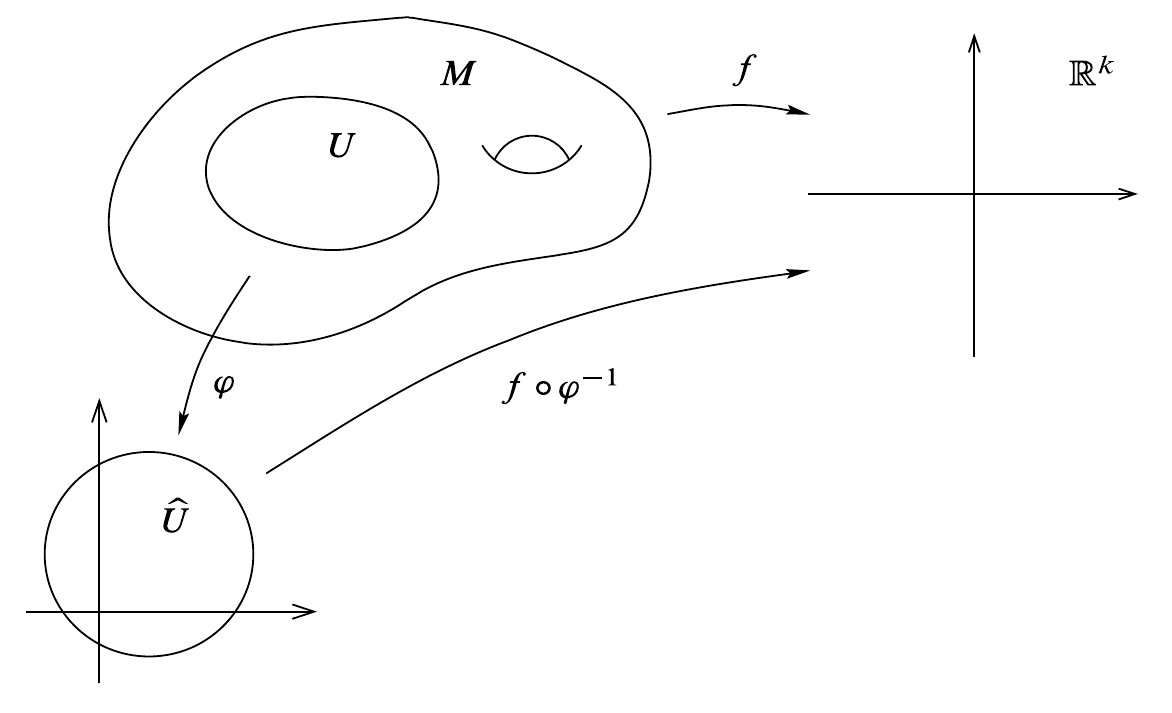
\includegraphics[scale = 0.35]{chapter02/c2f1.png}
\end{center}

\dfn Given a function $f:M\ra \Rk$ and a chart $(U,\vphi)$ for $M$, the function $\wh f:\vphi(U)\ra \Rk$ defined by $\wh f(x) = f\circ\vphi\inv(x)$ is called the \textbf{\textit{coordinate representation of f}}.

\dfn Let $M,\,N$ be smooth manifolds, and let $F:M\ra N$ be any map. We say that $F$ is a \textbf{\textit{smooth map}} if for every $p\in M$, there exist smooth charts $(U,\vphi)$ containing $p$ and $(V,\psi)$ containing $F(p)$ such that $F(U)\seq V$ and the composite map $\psi\circ\vphi\inv$ is smooth from $\vphi(U)$ to $\psi(V)$.

\begin{center}
    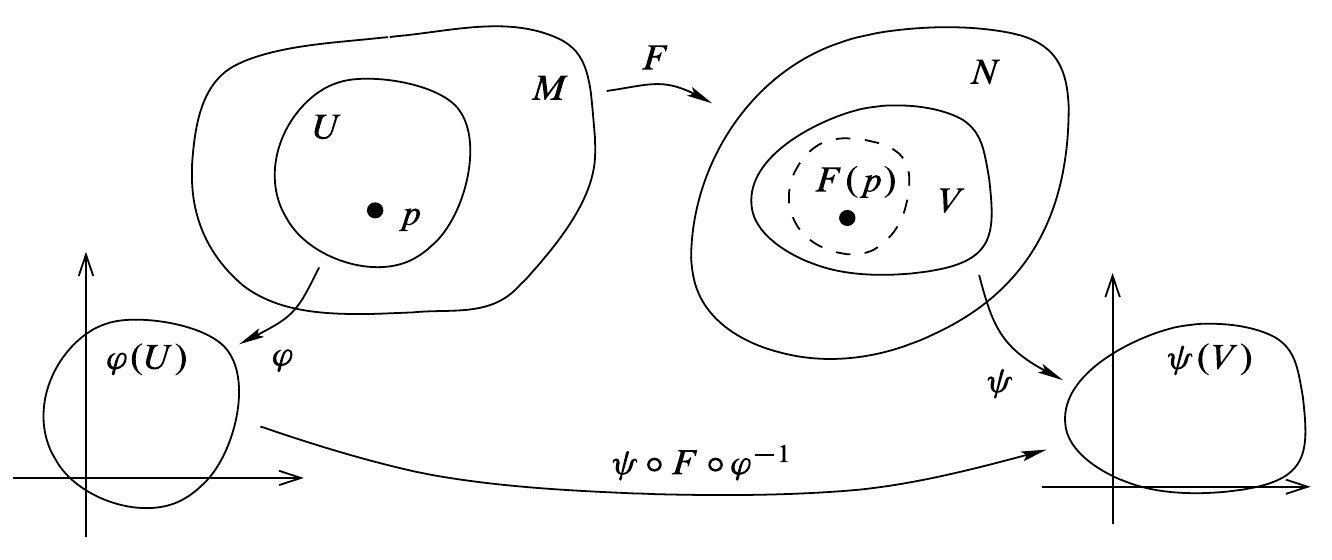
\includegraphics[scale = 0.4]{chapter02/c2f2.png}
\end{center}

\setcounter{thm}{3}

\begin{prop}
Every smooth map is continuous
\end{prop}

\begin{prop}[Equivalent Characterizations of Smoothness]
Suppose $M$ and $N$ are smooth manifolds with or without boundary, and $F:M\ra N$ is a map. Then $F$ is smooth if and only if either of the following conditions is satisfied:
\begin{enumerate}
    \item For every $p\in M$, there exist smooth charts $(U,\vphi)$ containing $p$ and $(V, \psi)$ containing $F(p)$ such that $U\cap F\inv(V)$ is open in $M$ and the composite map $\psi\circ F\circ \vphi\inv$ is smooth from $\vphi(U\cap F\inv(V))$ to $\psi(V)$.
    \item $F$ is continuous and there exist smooth atlases $\{(U_\al, \vphi_\al)\}$ and $\{(V_\be, \psi_\be)\}$ for $M$ and $N$, respectively, such that for each $\al$ and $\be$, $\psi_\be\circ F\circ\vphi_\al\inv$ is a smooth map from $\vphi_\al(U_\al\cap F\inv(V_\be))$ to $\psi_\be(V_\be)$.
\end{enumerate}
\end{prop}

\begin{prop}[Smoothness is Local]Let $M$ and $N$ be smooth manifolds with or without boundary, and let $F:M\ra N$ be a map.
\begin{enumerate}
    \item If every point $p\in M$ has a neighborhood $U$ such that the restriction $F|_U$ is smooth, then $F$ is smooth.
    \item Conversely, if $F$ is smooth, then its restriction to every open subset is smooth.
\end{enumerate}
\end{prop}

\setcounter{thm}{7}

\begin{cor}[\hl{Gluing Lemma for Smooth Maps}]
Let $M$ and $N$ be smooth manifolds with or without boundary, and let $\{U_\al\}_{\al\in A}$ be an open cover of $M$. Suppose that for each $\al\in A$, we are given a smooth map $F_\al:U_\al\ra N$ such that the maps agree on overlaps: $\ev{F_\al}{U_\al\cap U_\be} = \ev{F_\be}{U_\al\cap U_\be}$ for all $\al$ and $\be$. Then there exists a unique smooth map $F:M\ra N$ such that $\ev{F}{U_\al} = F_\al$ for each $\al\in A$.
\end{cor}

\setcounter{thm}{9}

\begin{prop}Let $M$, $N$, and $P$ be smooth manifolds with or without boundary.
\begin{enumerate}
    \item Every constant map $c:M\ra n$ is smooth.
    \item The identity map of $M$ is smooth.
    \item \hl{If $C\seq M$ is an open submanifold with or without boundary, then the inclusion map $U\into M$ is smooth.}
    \item If $F:M\ra N$ and $G:N\ra P$ are smooth, then so is $G\circ F:M\ra P$.
\end{enumerate}
\end{prop}

\setcounter{thm}{11}

\begin{prop}
Suppose $M_1,\ldots,M_k$ and $N$ are smooth manifolds with or without boundary, such that at most one of $M_1,\ldots,M_k$ has nonempty boundary. For each $i$, let $\pi_I:M_1\x \cdots\x M_k\ra M_i$ denote the projection onto the $M_i$ factor. A map $F:N\ra M_1\x \cdots \x M_k$ is smooth if and only if each of the component maps $F_i = \pi_i\circ F:N\ra M_i$ is smooth.
\end{prop}

\dfn If $M$ and $N$ are smooth manifolds with or without boundary, a \textbf{\textit{diffeomorphism from M to N}} is a smooth bijective map $F:M\ra N$ that has a smooth inverse.

\setcounter{thm}{17}

\begin{thm}[Diffeomorphism Invariance of Dimension]
A nonempty smooth manifold of dimension $m$ cannot be diffeomorphic to an $n$-dimensional smooth manifold unless $m = n$
\end{thm}

\begin{thm}[Diffeomorphism Invariance of Boundary]
Suppose $M$ and $N$ are smooth manifolds with boundary and $F:M\ra N$ is a diffeomorphism. Then $F(\bd M) = \bd N$, and $F$ restricts to a diffeomorphism from $\Int(M)$ to $\Int(N)$.
\end{thm}
\newpage
\subsection{Partitions of Unity}\nl

\begin{lem}
The functions $f:\R\ra \R$ defined by
\[f(t) = \begin{cases} e^{-\frac{1}{t}}, & t > 0,\\ 0. & t\leq 0,\end{cases}\]
is smooth.
\end{lem}

\begin{lem}
Given any real numbers $r_1$ and $r_2$ such that $r_1 < r_2$, there exists a smooth function $h:\R\ra \R$ such that $h(t) \equiv 1$ for $t\leq r_1$, $0 < h(t) < 1$ for $r_1 < t < r_2$, and $h(t) \equiv 0$ for $t\geq r_2$.
\end{lem}

\begin{proof}
Let $f$ be the function of the previous lemma, and set 
\[h(t) = \frac{f(r_2 - t)}{f(r_2 - t) + f(t - r_1)}.\]
Then the denominator is always positive since $r_2 \neq r_1$ and either $r_2 - t$ or $t - r_1$ will always be positive, and the rest follows form the properties of $f$.
\end{proof}

\begin{lem}
Given any positive real numbers $r_1 < r_2$, there is a smooth function $H:\Rn\ra \R$ such that $H \equiv 1$ on $\ol B_{r_1}(0), 0 < H(x) < 1$ for all $x \in B_{r_2}(0)\backslash \ol B_{r_1}(0)$, and $H\equiv 0$ on $\Rn \backslash B_{r_2}(0)$.
\end{lem}

\dfn The function $H$ constructed in the previous lemma is an example of a \df{smooth bump function}, a smooth real-valued function that is equal to 1 on a specified set and is zero outside a specified neighborhood of that set.

\dfn If $f$ is any real-valued or vector-valued function on a topological space $M$, the \df{support of f}, denoted $\supp(f)$, is the \ul{closure of the set of points} where $f$ is nonzero:
\[\supp(f) = \ol{\{p\in M\ :\ f(p)\neq 0\}}\]
A function $f$ is said to be \df{compactly supported} if $\supp(f)$ is a compact set.

\dfn Suppose that $M$ is a topological space, and let $\XX = (X_\al)_{\al\in A}$ be an arbitrary open cover of $M$. A \df{partition of unity subordinate to $\boldsymbol{X}$} is an indexed family $(\psi_\al)_{\al\in A}$ of continuous functions $\psi_\al:M\ra \R$ with the following properties:
\begin{enumerate}[(i)]
    \item $0 \leq \psi_\al(x)\leq 1$ for all $\al\in A$ and all $x\in M$.
    \item $\supp(\psi_\al) \seq X_\al$ for each $\al\in A$.
    \item The family of supports $(\supp(\psi_\al))_{\al\in A}$ is locally finite. 
    \item $\sum_{\al\in A}\psi_\al(x) = 1$ for all $x\in M$.
\end{enumerate}
If $M$ is a smooth manifold with or without boundary, a \df{smooth partition of unity} is one for which each of the unctions $\psi_\al$ is smooth.

\begin{thm}[Existence of Partitions of Unity]
Suppose $M$ is a smooth manifold with or without boundary, and $\XX = (X_\al)_{\al\in A}$ is any indexed open cover of $M$. Then there exists a smooth partition of unity subordinate to $\XX$.
\end{thm}

\dfn If $M$ is a topological space, $A\seq M$ is a closed subset, and $U\seq M$ is an open subset containing $A$, a continuous function $\psi:M\ra \R$ is called a \df{\hl{bump function for A supported in U}} if $0 \leq \psi \leq 1$ on $M$, $\psi \equiv 1$ on $A$, and $\supp(\psi)\seq U$.

\setcounter{thm}{24}

\begin{prop}[Existence of Smooth Bump Functions]
Let $M$ be a smooth manifold with or without boundary. For any closed subset $A\seq M$ and any open subset $U$ containing $A$, there exists a smooth bump function for $A$ supported in $U$.
\end{prop}

\dfn Suppose that $M$ and $N$ are smooth manifolds with or  without boundary, and $A\seq M$ is an arbitrary subset. We say that a map $F:A\ra N$ is \df{smooth on A} if it has a smooth extension in a neighborhood of each point: that is, if for every $p\in A$ there is an open subset $W\seq M$ containing $p$ an a smooth map $\td F:W\ra N$ whose restriction to $W\cap A$ agrees with $F$.

\begin{lem}[\hl{Extension Lemma for Smooth Functions}]
Suppose $M$ is a smooth manifold with or without boundary, $A\seq M$ a closed subset, and $f:M\ra \Rk$ is a smooth function. For any open subset $U$ containing $A$, there exists a smooth function $\td f:M\ra \Rk$ such that $\td f_A = f$ and $\supp(\td f)\seq U$.
\end{lem}

\dfn Suppose that $M$ is a topological space. An \df{exhaustion function for M} is a continuous function $f:M\ra \R$ with the property that the set $f\inv((-\infty, c])$ (called a \df{sublevel set of f}) is compact for each $c\in \R$. For an example consider the function $f:\Rn\ra \R:x\mapsto |x|^2$.

\setcounter{thm}{27}

\begin{prop}[Existence of Smooth Exhaustion Functions]
Every smooth manifold with or without boundary admits a smooth, positive exhaustion function.
\end{prop}

\begin{thm}[\hlb{Level Sets of Smooth Functions}]
Let $M$ be a smooth manifold. If $K$ is any closed subset of $M$, there is a smooth, nonnegative function $f:M\ra \R$ such that $f\inv(0) = K$.
\end{thm}










